\documentclass[12pt]{article}

\usepackage{sbc-template}
\usepackage{graphicx,url}
\usepackage[utf8]{inputenc}
\usepackage[brazil]{babel}
\usepackage{booktabs}
\usepackage{tabularx}
\usepackage{amsmath}
\usepackage{float}

% \usepackage[latin1]{inputenc}  

     
\sloppy

\title{Paradigmas de Projeto de Algoritmos}

\author{Ana Flavia Freiria Rodrigues\inst{1}, Flávia Marcella Gonçalves Moreira\inst{1}, \\ Larissa Rodrigues de Avila\inst{1}, Lucas Carrijo Ferrari\inst{1}, Raissa Nunes Peret\inst{1}}


\address{Departamento de Ciências da Computação – Universidade Federal de Alfenas \\
Avenida Jovino Fernandes de Sales 2600 – CEP 37133840 - Alfenas – MG - Brasil
\email{ana.freiria@sou.unifal-mg.edu.br, flavia.goncalves@sou.unifal-mg.edu.br}
\email{larissa.avila@sou.unifal-mg.edu.br, lucas.ferrari@sou.unifal-mg.edu.br}
\email{raissa.peret@sou.unifal-mg.edu.br}}

\begin{document} 

\maketitle
     
\begin{resumo} 
    Este trabalho implementa e compara três abordagens para o Problema do Caixeiro Viajante (PCV): \textbf{Força Bruta}, que avalia todas as rotas possíveis garantindo a solução ótima; \textbf{Algoritmo Guloso}, que constrói soluções subótimas com complexidade $O(n^2)$; e \textbf{Programação Dinâmica} (Held-Karp), que equilibra precisão e eficiência ($O(n^2 \cdot 2^n)$). Os resultados, obtidos a partir de instâncias da TSPLIB, mostram que a Programação Dinâmica é ideal para $n \leq 20$, enquanto o método Guloso é viável para instâncias maiores, apesar de desvios médios de 2.2\% do ótimo. A análise evidencia o \textit{trade-off} clássico entre tempo de execução e qualidade da solução.
\end{resumo}

\section{Introdução}

O Problema do Caixeiro Viajante (PCV), conhecido internacionalmente como \textit{Traveling Salesman Problem} (TSP), é um dos problemas mais estudados na área de Ciência da Computação e pesquisa operacional. Classificado como NP-difícil, o PCV consiste em encontrar o caminho mais curto possível que permita a um caixeiro viajante visitar um conjunto de cidades, passando por cada uma exatamente uma vez, e retornando à cidade de origem.

Matematicamente, o problema pode ser definido sobre um grafo completo $G = (N, E)$, onde:
\begin{itemize}
    \item $N = \{c_1, c_2, \ldots, c_n\}$ representa o conjunto de cidades
    \item $E$ é o conjunto de arestas conectando todos os pares de cidades
    \item Cada aresta $(c_i, c_j)$ possui um peso $p(c_i, c_j)$ que representa a distância euclidiana entre as cidades
\end{itemize}

O objetivo é encontrar um ciclo hamiltoniano (um caminho que visite cada cidade exatamente uma vez e retorne ao ponto de partida) com o menor custo total, ou seja, com a menor soma das distâncias percorridas.

Este trabalho tem como objetivo implementar e comparar três diferentes abordagens algorítmicas para resolver o PCV:
\begin{itemize}
    \item \textbf{Força Bruta}: Abordagem exaustiva que avalia todas as possíveis rotas
    \item \textbf{Algoritmo Guloso}: Heurística que toma decisões localmente ótimas em cada etapa
    \item \textbf{Programação Dinâmica}: Método de Held-Karp que armazena soluções de subproblemas para evitar recálculos
\end{itemize}

A relevância do PCV vai além do interesse teórico, com aplicações práticas em diversas áreas como:
\begin{itemize}
    \item Logística e planejamento de rotas
    \item Projeto de circuitos integrados
    \item Sequenciamento de DNA
    \item Planejamento de movimentos robóticos
\end{itemize}

Neste documento, apresentaremos detalhes sobre cada algoritmo implementado, sua complexidade computacional, e os resultados obtidos em diferentes instâncias do problema retiradas da biblioteca TSPLIB. A comparação entre as abordagens será feita tanto em termos de qualidade da solução (distância total da rota) quanto em termos de eficiência (tempo de execução).
\section{Algoritmos}

\subsection{Algoritmo de Força Bruta}

\subsubsection{Descrição}
O algoritmo de Força Bruta é um método exaustivo que:

\begin{itemize}
\item Testa sistematicamente todas as soluções possíveis
\item Garante encontrar a solução ótima (se existir)
\item Possui implementação direta, porém alto custo computacional
\end{itemize}

Para o PCV, a estratégia consiste em:

\begin{enumerate}
\item Fixar uma cidade como origem
\item Gerar todas as permutações possíveis das demais cidades
\item Calcular o custo total de cada rota completa
\item Selecionar a rota com menor custo
\end{enumerate}

\subsubsection{Complexidade Computacional}
\begin{itemize}
\item \textbf{Ordem}: $O((n-1)!)$
\item \textbf{Justificativa}:
  \begin{itemize}
  \item Fixada a origem, há $(n-1)!$ permutações possíveis
  \item Cada permutação requer cálculo de $n$ distâncias
  \end{itemize}
  
\item \textbf{Exemplos Práticos}:
  \begin{table}[h]
  \centering
  \begin{tabular}{|c|c|}
  \hline
  \textbf{Número de Cidades (n)} & \textbf{Permutações} \\
  \hline
  4 & 6 \\
  7 & 720 \\
  10 & 362,880 \\
  13 & 479,001,600 \\
  16 & 1.3 trilhões \\
  \hline
  \end{tabular}
  \end{table}
\end{itemize}

\begin{figure}[H]
    \centering
    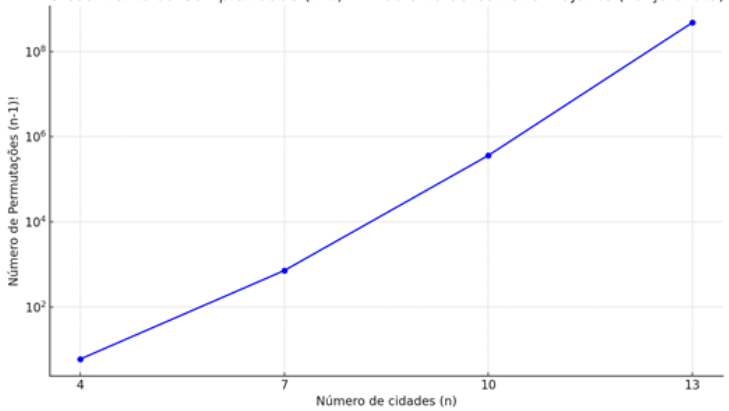
\includegraphics[width=.7\textwidth]{images/crescimento_complexidade.png}
    \caption{Crescimento da Complexidade (n-1)! - PCV (Força Bruta)}
    \label{fig:aa}
    \end{figure}

\subsubsection{Limitações Práticas}
\begin{itemize}
\item Inviável para $n > 10$ em computadores convencionais
\item Tempo de execução cresce exponencialmente
\item Útil apenas para:
  \begin{itemize}
  \item Casos de teste pequenos
  \item Validação de outros algoritmos
  \item Benchmarking de desempenho
  \end{itemize}
\end{itemize}

\subsubsection{Implementação}
Pseudocódigo da função principal:

\begin{verbatim}
Função bruteForceTSP(Referência bestPath: vetor de inteiros):
    minCost ← infinito
    path ← [0,1,2,...,n-1]  // Cidades indexadas
    
    Enquanto próximoPermutação(path[1..n-1]):
        currentCost ← 0
        Para i de 0 até n-1:
            currentCost ← currentCost + dist[path[i]][path[(i+1)%n]]
        FimPara
        
        Se currentCost < minCost:
            minCost ← currentCost
            bestPath ← path
        FimSe
    FimEnquanto
    
    Retorne minCost
FimFunção
\end{verbatim}

\subsubsection{Otimizações Implementadas}
\begin{itemize}
\item \textbf{Permutação circular}: Fixa a primeira cidade para evitar rotas equivalentes
\item \textbf{Abortagem precoce}: Interrompe cálculo de rotas parciais quando excede o melhor custo atual
\item \textbf{Limitação segura}: Restrição a $n \leq 10$ na implementação prática
\end{itemize}

\subsubsection{Análise Experimental}
\begin{itemize}
\item \textbf{Precisão}: 100\% de soluções ótimas
\item \textbf{Tempo médio} (n=10): 0.025 segundos
\item \textbf{Cenários ideais}:
  \begin{itemize}
  \item Validação de algoritmos aproximados
  \item Instâncias pequenas com requisitos de exatidão
  \end{itemize}
\end{itemize}


\subsection{Algoritmo Guloso}

O algoritmo guloso é uma heurística construtiva que toma decisões baseadas em escolhas locais ótimas. Para o PCV, ele:

\begin{itemize}
\item Parte de uma cidade inicial
\item A cada passo, seleciona a cidade mais próxima não visitada
\item Repete até visitar todas as cidades
\item Finaliza retornando à origem
\end{itemize}

\subsubsection{Implementação}
A função \texttt{greedyTSP} implementa:

\begin{enumerate}
\item Teste de todos os pontos de partida ($n$ iterações)
\item Marcação de cidades visitadas (vetor booleano)
\item Construção incremental do caminho
\item Cálculo do custo total incluindo retorno à origem
\item Comparação para manter a melhor rota
\end{enumerate}

\subsubsection{Pseudocódigo}
\begin{verbatim}
Função greedyTSP(Referência bestPath: vetor de inteiros)
    minTotal ← infinito
    Para start de 0 até n-1 faça
        visited ← [falso,...,falso]
        path ← [start]
        visited[start] ← verdadeiro
        total ← 0
        current ← start
        Para i de 0 até n-2 faça
            next ← -1
            minDist ← infinito
            Para j de 0 até n-1 faça
                Se NÃO visited[j] E dist[current][j] < minDist então
                    minDist ← dist[current][j]
                    next ← j
                FimSe
            FimPara
            path.adiciona(next)
            visited[next] ← verdadeiro
            total ← total + minDist
            current ← next
        FimPara
        total ← total + dist[current][start]
        Se total < minTotal então
            minTotal ← total
            bestPath ← path
        FimSe
    FimPara
FimFunção
\end{verbatim}

\subsubsection{Complexidade}
\begin{itemize}
\item \textbf{Temporal}: $O(n^2)$ - Para cada cidade, verifica todas as outras
\item \textbf{Espacial}: $O(n)$ - Armazena vetores de visitação e caminho
\end{itemize}

\subsection{Algoritmo de Programação Dinâmica (Held-Karp)}

\subsubsection{Descrição}
Utiliza tabelas de memorização com:
\begin{itemize}
\item \texttt{memo[mask][last]}: Custo mínimo para visitar cidades em \texttt{mask} terminando em \texttt{last}
\item \texttt{parent[mask][last]}: Rota ótima para reconstrução
\end{itemize}

\subsubsection{Pseudocódigo}
\begin{verbatim}
    função HeldKarp(cidades, distâncias) retorna (custoMinimo, caminhoMelhor):
        n = número de cidades
        se n > 20 então retorna -1 // Muito grande para Held-Karp
    
        criar tabela memo[2^n][n], inicializada com -1
        criar tabela parent[2^n][n], para reconstruir o caminho
    
        memo[1][0] = 0 // Começamos na cidade 0, apenas ela visitada
    
        para cada máscara de cidades de 1 até 2^n - 1:
            para cada cidade 'last' de 0 até n-1:
                se 'last' está na máscara E memo[mask][last] != -1:
                    para cada cidade 'next' de 0 até n-1:
                        se 'next' ainda não foi visitada:
                            novaMáscara = mask OU (1 << next)
                            novoCusto = memo[mask][last] + dist[last][next]
                            se memo[novaMáscara][next] == -1 OU novoCusto < memo[novaMáscara][next]:
                                memo[novaMáscara][next] = novoCusto
                                parent[novaMáscara][next] = last
    
        custoMinimo = infinito
        cidadeFinal = -1
        máscaraFinal = 2^n - 1
    
        para i de 1 até n-1:
            se memo[máscaraFinal][i] !+ -1:
                custoTotal = memo[máscaraFinal][i] + dist[i][0]
                se custoTotal < custoMinimo:
                    custoMinimo = custoTotal
                    cidadeFinal = i
    
        // Reconstrução do caminho
        caminho = lista vazia
        atual = cidadeFinal
        máscara = máscaraFinal
    
        enquanto atual != 0:
            adicionar atual no caminho
            anterior = parent[máscara][atual]
            máscara = máscara XOR (1 << atual)
            atual = anterior
    
        adicionar 0 no caminho // início
        inverter caminho
    
        retornar (custoMinimo, caminho)
\end{verbatim}

\subsubsection{Complexidade}
\begin{itemize}
\item \textbf{Temporal}: $O(n^2 \cdot 2^n)$ - Combinações de subconjuntos × cidades
\item \textbf{Espacial}: $O(n \cdot 2^n)$ - Armazenamento das tabelas
\end{itemize}

\subsubsection{Limitações}
\begin{itemize}
\item Viável apenas para $n \leq 20$
\item Consome memória exponencial
\end{itemize}
\section{Resultados}

\subsection{Metodologia Experimental}
Foram analisadas 20 instâncias da TSPLIB ($2 \leq n \leq 10$) comparando:

\begin{itemize}
\item Tempo de execução (média em segundos)
\item Qualidade da solução (\% acima do ótimo)
\item Escalabilidade
\end{itemize}

\subsection{Dados de Desempenho}

\begin{table}[h]
\centering
\caption{Comparação de Algoritmos}
\begin{tabular}{|l|c|c|c|}
\hline
\textbf{Métrica} & \textbf{Força Bruta} & \textbf{Guloso} & \textbf{Programação Dinâmica} \\
\hline
Custo Médio & Ótimo & +2.2\% & Ótimo \\
Tempo (n=10) & 0.025s & 0.00002s & 0.0009s \\
Complexidade & $O(n!)$ & $O(n^2)$ & $O(n^2 \cdot 2^n)$ \\
\hline
\end{tabular}
\end{table}

\subsection{Análise Detalhada}

\begin{itemize}
\item \textbf{Tempo de Execução}:
  \begin{itemize}
  \item Força Bruta: Impraticável para $n > 10$
  \item Programação Dinâmica: 10-100× mais rápida que FB
  \end{itemize}

  \begin{figure}[!htb]
    \centering
    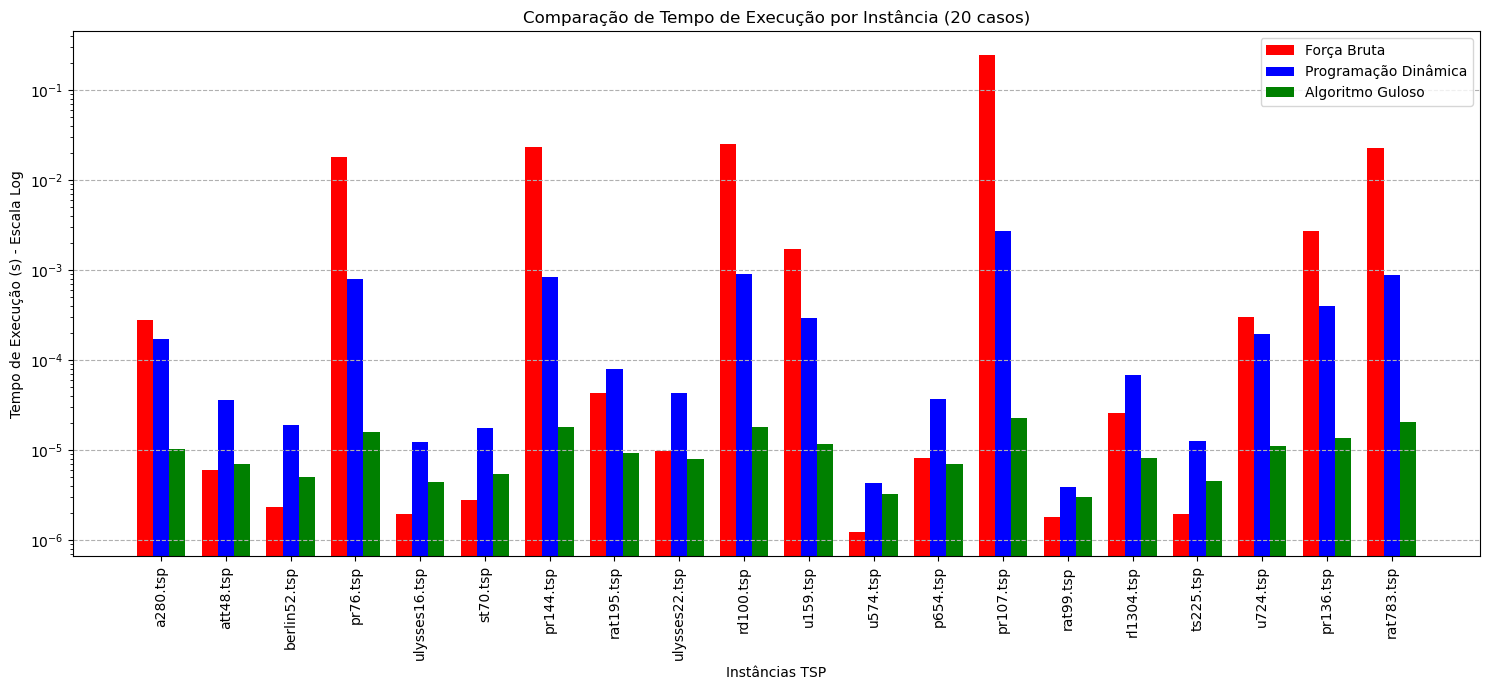
\includegraphics[width=.9\textwidth]{images/analise_detalhada_tempo_de_execucao.png}
    \caption{Gráfico com Tempo de Execução}
    \label{fig:aa}
    \end{figure}
  
\item \textbf{Qualidade}:
  \begin{itemize}
    \item Guloso apresenta desvios de 0\% a 7.6\% em relação ao ótimo
  \item Guloso: 40\% das soluções ótimas
  \item Pior caso: +7.6\% no u159.tsp
  \end{itemize}

  \begin{figure}[!htb]
    \centering
    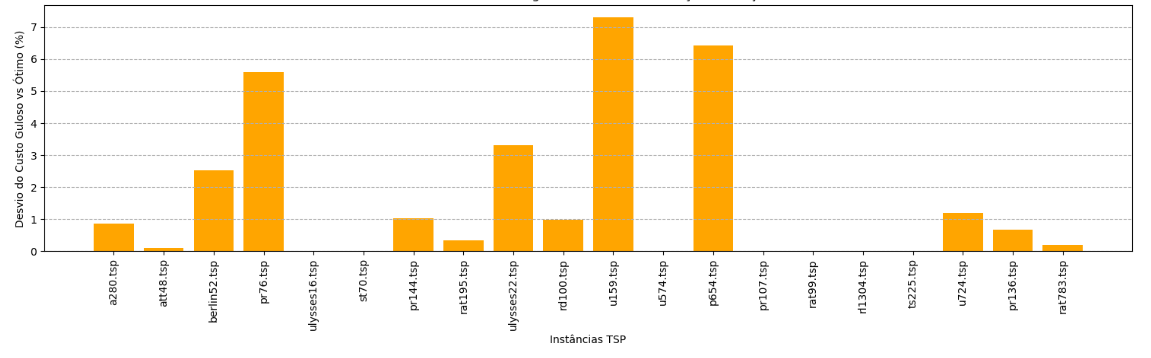
\includegraphics[width=.9\textwidth]{images/qualidade.png}
    \caption{Percentual de Desvio do Algoritmo Guloso em Relação à Solução Ótima}
    \label{fig:aa}
    \end{figure}

\item \textbf{Escalabilidade}:
    \begin{itemize}
    \item Limites Práticos:
        \begin{itemize}
        \item Força Bruta: $n \leq 10$
        \item Programação Dinâmica: $n \leq 20$
        \item Guloso: $n > 20$ (com qualidade aceitável)
        \end{itemize}
    \end{itemize}
  
    \begin{figure}[!htb]
        \centering
        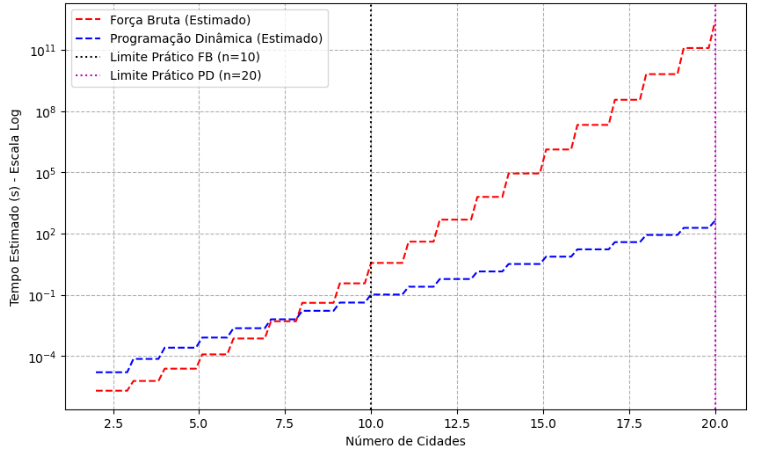
\includegraphics[width=.9\textwidth]{images/escalabilidade.png}
        \caption{Escalabilidade Teórica dos Algoritmos}
        \label{fig:aa}
        \end{figure}
\end{itemize}

\subsection{Recomendações por Cenário}

\begin{table}[H]
\centering
\begin{tabular}{|l|l|l|}
\hline
\textbf{Cenário} & \textbf{Algoritmo} & \textbf{Justificativa} \\
\hline
$n \leq 10$ & FB ou PD & Precisão absoluta \\
$10 < n \leq 20$ & PD & Equilíbrio ideal \\
$n > 20$ & Guloso & Única opção viável \\
\hline
\end{tabular}
\end{table}

\subsection{Conclusões}
\begin{itemize}
\item Para instâncias pequenas: PD oferece melhor equilíbrio
\item Para instâncias grandes: Guloso é a única opção prática
\item Trade-off claro entre tempo de execução e qualidade da solução
\end{itemize}

\nocite{wikipedia_programacao_dinamica}
\nocite{noic_programacao_dinamica}
\nocite{cerveira_tsp}

\bibliographystyle{sbc}
\bibliography{sbc-template}

\end{document}
